\documentclass[paper=a4]{scrartcl}

\usepackage{basis}

% Metadata.
\newcommand{\Title}{Spell Checker for EiffelStudio}
\newcommand{\Author}{Benjamin Fischer}
\newcommand{\Date}{17 February 2013}
\title{\Title}
\author{\Author}
\date{\Date}

\begin{document}

% Set title.
\begin{center}
\vspace*{2em}
\textbf{\LARGE \Title} \\
\vspace{2em}
\emph{\large Software Engineering Laboratory: Open-Source EiffelStudio} \\
\vspace{1em}
\end{center}
\begin{flushleft}
Semester project by \Author \hfill Student number: 10-916-971 \\
Supervised by Julian Tschannen \hfill ETH Computer Science \\
Prof. Dr. Bertrand Meyer \hfill \Date
\vspace{2em}
\end{flushleft}

\section{Requirements engineering}

\subsection{Introduction: Purpose and scope of the system}

EiffelStudio is a development environment for the Eiffel programming language. It currently does not have a spell checker. Thus, the idea of this project is to integrate a spell checker into EiffelStudio in order to check the spelling of class and feature comments. The first part of the project is about developing a spell checker library in Eiffel, which is used in the second part to integrate a spell checker tool into EiffelStudio.

\subsection{Proposed system}

The first part with the spell checker library is the core, while the possible additional features of the second part are only nice to have.

\subsubsection{Functional requirements}

\paragraph{Part 1: Eiffel library to check the spelling of strings}

\begin{itemize}
\item Select a spell checking back end
\item Select the language
\item Check the correctness of a word (ASCII or UTF32)
\item Check the correctness of a sentence (ASCII or UTF32)
\item Get suggestions for an incorrect word
\item Get suggestions for incorrect words in a sentence
\item Support a user dictionary and an ignore list, both of which can be created, added words to, loaded and stored as well as queried for list of words
\item The spell checker library should make multiple back ends possible. Support for at least one back end should be implemented already, for example GNU Aspell using its command-line interface.
\end{itemize}

\paragraph{Part 2: Spell checker tool for EiffelStudio}

\begin{itemize}
\item Minimum requirements
\begin{itemize}
\item Push a button to launch the spell checker
\item Check class and feature comments
\item Show spelling suggestions as warnings in EiffelStudio’s error list
\end{itemize}
\item Possible additional features (in no particular order)
\begin{itemize}
\item Optional requirements
\begin{itemize}
\item Check a class name (ignoring a possible class prefix)
\item Check feature names, argument names and names of local variables
\item Check the content of manifest strings
\item Check tag names of assertion and note clauses
\end{itemize}
\item Fancy requirements
\begin{itemize}
\item Ability to add words to a user dictionary
\item Ability to ignore words for a specific project
\item Automatic spell checking after saving a file
\item Show spelling suggestions and spell checker options in its own tool
\item Correct class text automatically when spelling suggestion is selected
\end{itemize}
\end{itemize}
\end{itemize}

\subsubsection{Nonfunctional requirements}

\begin{itemize}

\item The source code meets the style guidelines for Eiffel as summarised by Marcel Kessler in \Work{DO IT WITH STYLE – A Guide to the Eiffel Style} at \url{http://se.inf.ethz.ch/courses/2012b_fall/eprog/additional_materials/style_guideline_summary.pdf}.

\item A student in the second year of computer science at ETH should be able to understand and use the spell checker library by the end of one working day.

\item Most of the source code should document itself in form of a good programming style with contracts, comments, tests and usage examples. The documentation of the project with requirements engineering, design and testing is summarised and delivered with this final report.

\item The Eiffel source code should be void-safe.

\end{itemize}

% User interface and human factors
% Documentation
% Hardware considerations
% Performance characteristics
% Error handling and extreme conditions
% System interfacing
% Quality issues
% System modifications
% Physical environment
% Security issues
% Resources and management issues

% Object model

% Class diagrams
% Entity Objects
% Boundary Objects
% Control Objects

% Dynamic model

% Sequence chart diagrams
% State chart diagrams

% User Interface

\section{Design}

\subsection{Design goals}

The main objectives of the software in order of decreasing priority are as follows.

\begin{enumerate}

\item Maintainability. Both the spell checker library and its integration into EiffelStudio will be developed from scratch. The library might be used by other developers who directly use the source code. For this reasons, it is particularly important to prepare the software for changes. The most important objective is to make the software maintainable and hence easy to understand as well as improve. It should be possible to add new back ends without significantly changing the other parts of the system.

\item Usability. The library should have an intuitive interface for other developers using it. There should be clear documentation in both formal language like good contracts and informal language in comments. What is more, usage examples for the library should be provided.

\end{enumerate}

% Introduction
% Provide a brief overview of the software architecture and the design goals

% Purpose of the System
% Design Goals
% Definitions, Acronyms, and Abbreviations
% References

% Overview

% Current Software Architecture

% Describes the architecture of the system being replaced.
% If there is no previous system, give a survey of current architecture for similar systems.

% Proposed Software Architecture
% Document the system design model

% Overview
% Present a bird's eye view of the software architecture and briefly describe
% the assignment of functionality to each subsystem

% Subsystem Decomposition
% Describe the decomposition into subsystems and the responsibilities of each

% Hardware/Software Mapping
% Describe how the subsystems are assigned to hardware and off-the-shelf components.

% Persistent Data Management
% Describe the persistent data stored by the system and the data management
% infrastructure required for it.

% Access Control and Security
% Describe the user model of the system in terms of an access matrix.

% Global Software Control
% Describe how the global software control is implemented. In particular,
% this section should describe how requests are initiated and how subsystems
% synchronize. This section should also address synchronization and concurrency
% issues.

% Boundary Conditions
% Describe the start-up, shutdown, and error behavior of the system. If
% use cases are discovered for system administration, these should be
% included in the requirements analysis document.

% Subsystem Services
% Describe the services provided by each subsystem in terms of operations.
% This section serves as a reference for teams for the boundaries between
% their subsystems.

% Glossary

\subsection{Detailed design}

In the following, the spell checker library as seen in the BON class diagram of figure~\ref{Class diagram} is presented. We give an overview of the structure.

\begin{figure}
\centering
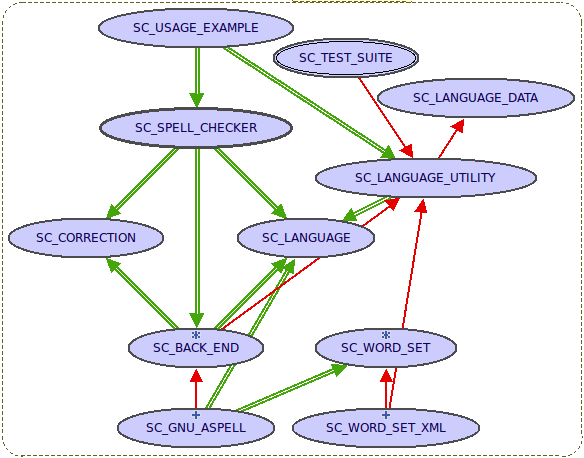
\includegraphics[width=\textwidth]{object_model.png}
\caption{BON class diagram of the spell checker library}
\label{Class diagram}
\end{figure}

Making use of a facade pattern, the central functionality comes together at the class \Code{SC_SPELL_CHECKER}. It has an associated language represented by \Code{SC_LANGUAGE} in which the current spell checking is happening. The results of checking the spelling of words are given as objects of the type \Code{SC_CORRECTION}, which encapsulates a correction with suggestions for replacements if any. The service of a raw spell checker is abstracted into the deferred class \Code{SC_BACK_END}. Its only effective descendant at the moment is \Code{SC_GNU_ASPELL} for the GNU Aspell spell checker, following an adapter pattern.

For the need of user and ignore dictionaries, the deferred class \Code{SC_WORD_SET} provides an interface for a persistent set of words, realised by an effective heir \Code{SC_WORD_SET_XML} for an XML file format. With reusability in mind, general text processing queries are kept in the class \Code{SC_LANGUAGE_UTILITY}, which frequently serves as an ascendant for implementation inheritance. The raw data of the required Unicode properties is found in its parent \Code{SC_LANGUAGE_DATA}. The class \Code{SC_USAGE_EXAMPLE} gives source code examples of how to use the spell checker library. At the same time, it serves as a demonstration and tests the whole system. Finally, tests of the more hidden parts of the library are collected in the class \Code{SC_TEST_SUITE}.

% Introduction

% Class Diagrams
% Package 1
% Package 2

% OCL Specifications
% Class Invariants
% Method Specifications

% Sequence Diagrams

% Design Patterns

\section{Library guide}

This short user guide explains how to use the spell checker library and develop further back ends.

\subsection{Basic usage}

We introduce the usage of the spell checker library with an basic example taken from the class \Code{SC_USAGE_EXAMPLE}, namely the feature \Code{use_basics} as reproduced in listing~\ref{usage}. First of all, we create a default spell checker object. This instantiates a default back end and uses its default language. Next, we make sure the language for the spelling is British English and check a word. If this succeeds, we would like to know whether the spelling is correct. If the word is spelled incorrectly, then there are possibly suggestions to replace the word with. Note that the word can be misspelt and no suggestions are found. Therefore, one normally wishes to distinguish three cases: correct, incorrect with suggestions and incorrect without suggestions. Please see the class \Code{SC_USAGE_EXAMPLE} for more examples.

\lstinputlisting[caption={Basic usage of the spell checker taken from the examples in \Code{SC_USAGE_EXAMPLE}}, label=usage]{use_basics.e}

The class \Code{SC_SPELL_CHECKER} provides the commands
\begin{itemize}
\item \Code{check_word (word: READABLE_STRING_32)}
\item \Code{check_words (words: LIST [READABLE_STRING_32])}
\item \Code{check_text (text: READABLE_STRING_32)}
\end{itemize}
to check the spelling of a single word, all words in a list or a whole text, respectively. In order to check the kind and success of the last such check, there exist the corresponding predicates \Code{is_word_checked}, \Code{are_words_checked} and \Code{is_text_checked}. The results are offered by the queries
\begin{itemize}
\item \Code{last_word_correction: SC_CORRECTION}
\item \Code{last_words_corrections: LIST [SC_CORRECTION]}
\item \Code{last_text_corrections: LIST [SC_CORRECTION]}
\end{itemize}
on success of the respective check.

Moreover, the class \Code{SC_SPELL_CHECKER} provides operations on user and ignore dictionaries. Words in both of these kinds of dictionaries are always treated as correct. The difference is that the words in a user dictionary can be used by the spell checker as suggestions, while those in an ignore dictionary are never suggested as replacements. Both kinds of dictionaries can be extended with a word. Only when the corresponding store feature is called, such changes are made persistent. Finally, the words can be accessed through the type \Code{SET [READABLE_STRING_32]}.

\subsection{Extension and reuse}

The feature \Code{set_back_end} of \Code{SC_SPELL_CHECKER} can change the back end. The class \Code{SC_BACK_END} is deferred and has many features from \Code{SC_SPELL_CHECKER} mirrored with default implementations. Developers should note that any effective descendant of the class \Code{SC_BACK_END} must redefine one of the features \Code{check_word} or \Code{check_words}, since the default behaviour of both is to call the other.

The feature \Code{check_text} by default breaks the text into words and checks each word. The information about the word boundaries is preserved in the \Code{SC_CORRECTION} objects, so in particular their function \Code{substring} can be useful to extract the word. Depending on the language and back end used, this text segmentation may not be able to work as expected. In this case, the functions \Code{words_of_text} and \Code{is_word} should be redefined to adapt the text segmentation and word predicate to specific needs.

If a back end to be adapted does not support one of the kinds of dictionaries, the class \Code{SC_WORD_SET} and its heir \Code{SC_WORD_SET_XML} can be used. The interface guarantees the procedures \Code{extend} and \Code{prune} operating on the word set and \Code{load} and \Code{store} for the synchronisation with a persistent storage.

The class \Code{SC_BACK_END} has a query \Code{failure_message} in case a subsystem not in control of the program fails. The philosophy is that this message is empty if and only if there is no failure. For this reason, there should always be a nonempty message on failure.

The class \Code{SC_LANGUAGE_UTILITY} might prove useful in other contexts. It has simple facilities for text processing. In particular, the function \Code{words_of_text_with_punctuation} finds word limits in a Unicode text. It makes use of the given punctuation to recognise words like \Word{can’t} as a whole. To determine whether an arbitrary Unicode character belongs to the major general category of letters, it applies the function \Code{is_letter} in turn. Furthermore, the function \Code{first_newline} to find the first newline in a string takes various kinds of newlines into account.

\section{Validation}

As already mentioned, the spell checker library is tested by the classes \Code{SC_TEST_SUITE} and \Code{SC_USAGE_EXAMPLE}. They have already been developed from an early stage of the project to facilitate a test-driven development.

The spell checker tool for EiffelStudio is tested with the help of the class \Code{SC_EVOLVABLE}. This serves as an example of a piece of Eiffel source code to cover almost all the desired node types of an abstract syntax tree to be checked for spelling. The checked node types are the following. Note that only the names introduced by the code itself should be checked, but not others.

\begin{itemize}
\item Comments
\item String literals
\item Verbatim strings
\item Class names
\item Names of formal generic types
\item New name of renamed features
\item Feature names and possible synonyms
\item Names of formal parameters, local variables and components of tuples
\item Tags of indexing clauses
\item Tags of contracts of all kinds
\item Identifiers introduced by across loops
\item Identifiers introduced by tests for attached variables
\end{itemize}

% Introduction
% Describe the objectives and extent of the tests.

% Relationship to other documents
% Explain the relationship of the test plan to the other documents.

% System overview
% Focus on the structural aspects of testing, provide an overview of the system
% in terms of components that are tested during unit testing.

% Features to be tested/not to be tested
% Focus on the functional aspects of testing, identify all features and
% combinations of features to be tested.

% Also describe those features that are not to be tested and the reasons for
% not testing them.

% Pass/Fail criteria
% Specify the pass/fail criteria for the tests covered in this plan -
% description of functionality required in order for the client to accept the
% project for functional tests and the required pass-rate for unit and
% integration tests.

% Approach
% Describe the general approach to the testing process. Discuss the reasons for
% the selected integrated testing approach.
% A UML class diagram can be used to illustrate the dependencies between the
% individual tests and their involvement in integration tests.

% Testing materials (optional)
% Identify the resources that are needed for testing. Include the physical
% characteristics of the facilities, including hardware and software to support
% the tests.

% Functional tests
% The core of the test plan. List the test cases that are used during testing.

% Refactoring
% Describe refactoring done, justification and benefits.

\section{Deployment}

The spell checker library with its tool is now available as a part of EVE, a development environment built on top of EiffelStudio. It is thus distributed under the terms of the GNU General Public License. The library can be found in the folder \Path{library/spelling}, while all the required test data is located at \Path{library/spelling/tests}. The tool integrated into EVE is in the folder \Path{Eiffel/interface/graphical/tools/spelling}.

\end{document}
